\documentclass{article} % For LaTeX2e
\usepackage{nips13submit_e,times}
\usepackage{amsmath} % assumes amsmath package installed
\usepackage{amssymb}  % assumes amsmath package installed
\usepackage{bm}
%\usepackage{hyperref}
\usepackage{url}
\usepackage{tikz}
\usetikzlibrary{fit,shapes,arrows,automata}
\usepackage[titlenumbered,longend,ruled,linesnumbered]{algorithm2e}
%\documentstyle[nips13submit_09,times,art10]{article} % For LaTeX 2.09


% random helper commands
\DeclareMathOperator*{\argmin}{argmin}
\DeclareMathOperator*{\argmax}{argmax}
\DeclareMathOperator*{\proj}{proj}
\DeclareMathSymbol{\widehatsym}{\mathord}{largesymbols}{"62}
\newcommand\lowerwidehatsym{%
  \text{\smash{\raisebox{-1.3ex}{%
    $\widehatsym$}}}}
\newcommand\bowler[1]{%
  \mathchoice
    {\accentset{\displaystyle\lowerwidehatsym}{#1}}
    {\accentset{\textstyle\lowerwidehatsym}{#1}}
    {\accentset{\scriptstyle\lowerwidehatsym}{#1}}
    {\accentset{\scriptscriptstyle\lowerwidehatsym}{#1}}
}
\newcommand\mat[2]{\ensuremath{\left[\begin{array}{#1}#2\end{array}\right]}}
\newcommand\deriv[2]{\ensuremath{\frac{\partial #1}{\partial #2}}}
\newcommand{\overbar}[1]{\mkern 4mu\overline{\mkern-4mu#1\mkern-4mu}\mkern 4mu}

% notation
\def\change{ {\mathsmaller\Delta} }
\def\xmat{\uppercase}    \def\xmatstr{in uppercase}
\def\xvec{\vec}          \def\xvecstr{with an arrow}
\def\xuv{\hat}           \def\xuvstr{with a caret}
\def\xse{\bm}            \def\xsestr{in boldface}


\title{Automatic Modeling of Articulated Objects Using Screw Joint Trees}


\author{
Alex Burka and Daniel D.~Lee \\
Department of Electrical and Systems Engineering\\
University of Pennsylvania\\
Pennsylvania, PA 19104 \\
\texttt{\{aburka,ddlee\}@seas.upenn.edu} \\
}

% The \author macro works with any number of authors. There are two commands
% used to separate the names and addresses of multiple authors: \And and \AND.
%
% Using \And between authors leaves it to \LaTeX{} to determine where to break
% the lines. Using \AND forces a linebreak at that point. So, if \LaTeX{}
% puts 3 of 4 authors names on the first line, and the last on the second
% line, try using \AND instead of \And before the third author name.

\newcommand{\fix}{\marginpar{FIX}}
\newcommand{\new}{\marginpar{NEW}}

%\nipsfinalcopy % Uncomment for camera-ready version

\begin{document}


\maketitle

\begin{abstract}
  A difficult problem in semantic perception is articulated object modeling, that is, the pathway from three-dimensional input (e.g. stereo vision, structured light, LIDAR etc) to discovering the latent kinematic structure of an object with moving parts. In previous literature including \cite{Burka2013} and \cite{Sturm2009}, techniques are presented for using various joint models to assemble the most likely kinematic tree when presented with trajectory data. In this work, we focus on the more general screw joint model, which contains both revolute and prismatic joints as degenerate cases. We present an algorithm which models an articulated object using a tree of screw joints. The algorithm is tested in simulation and on data captured with a camera and augmented reality tags \cite{aruco}.
\end{abstract}

\section{Introduction}

\subsection{Motivation}
As robots become increasingly dextrous and equipped to interact with humans in human environments, there is a need to teach them to use human artifacts (tools, buildings, furniture, vehicles) in a natural and semantically appropriate way. Our work in this area focuses on understanding the kinematic structure of articulated objects (i.e. moving parts) in the environment. Humans rely heavily on intuition, pattern matching and experimentation for this task. For example, sitting down in a rental car may be momentarily disorienting, but a human driver already knows how to operate the pedals, gearshift and windshield wipers (the Prius being an exception). Door locks and radio controls are always different but can be found by analogy, or experimentation if necessary.

\subsection{Literature Review}
\cite{Sturm2009}, \cite{Aqvist1986}, \cite{Burka2013}

\subsection{Paper Outline}

\section{Articulated Objects as Screw Joint Trees}
Many everyday objects have several moving parts. The joints which connect two moving parts may be characterized by joint type and nmber of degrees of freedom (DoG). In this paper we will consider only joints with one degree of freedom. This covers most objects, though to represent some joints we would need two (such as a swivel chair which both rotates and extends) or even three (in the case of a ball-and-socket joint).

Furthermore, the only considered joint type will be the screw joint. Conceptually, a screw joint links two object parts $a$ and $b$ with one degree of freedom such that $b$ translates and rotates along the same axis with respect to $a$. The ratio between rotation and translation is the \emph{pitch}. Considering only this joint type is not so limiting as it seems, because the common joint types (i.e. those covered in \cite{Burka2013}) exist as degenerate cases. A prismatic joint is simply a screw joint with infinite pitch, whereas a revolute joint is a screw joint with zero pitch.

In general, an object with many moving parts must be modeled by a connected, directed graph where the vertices are object parts and the edges are joints.  Any node of indegree greater than unity has extra implied kinematic constraints. In this work these will be ignored, so all graphs in question will be trees. For an example, consider the two-axis translation table depicted in Figure \ref{fig:example} with its associated kinematic tree model. The long bars translate in two dimensions, and the red knobs control each axis. This tree contains both screw joints (the X knob with respect to the base, and the Y knob with respect to the X gantry) and prismatic joints, or infinite-pitch screw joints (the sliding gantries). Note that this is not the only possible model: the knobs could be modeled as connected to their respective gantries, where they would be pure revolute joints, or zero-pitch screws. Also, this model ignores the fact that the rotary motion of the knobs is causally related to the translation of the gantries: it is a kinematic model, not a dynamic one.

\begin{figure}[ht]
  \centering
  \begin{tikzpicture}[auto]
    \tikzstyle{node} = [draw, ellipse]

    \node (base) at (10,1.5) [node, accepting] {base};
    \node (xslide) [node, below of=base, node distance=4em] {X gantry};
    \node (yslide) [node, below of=xslide, node distance=4em] {Y gantry};
    \node (xknob) [node, left of=xslide, node distance=10em] {X control knob};
    \node (yknob) [node, left of=yslide, node distance=10em] {Y control knob};

    \draw [->] (base) -- node {Pr} (xslide);
    \draw [->] (xslide) -- node {Pr} (yslide);
    \draw [->] (base) -- node[above] {Sc} (xknob);
    \draw [->] (xslide) -- node[above] {Sc} (yknob);

    \node (image) {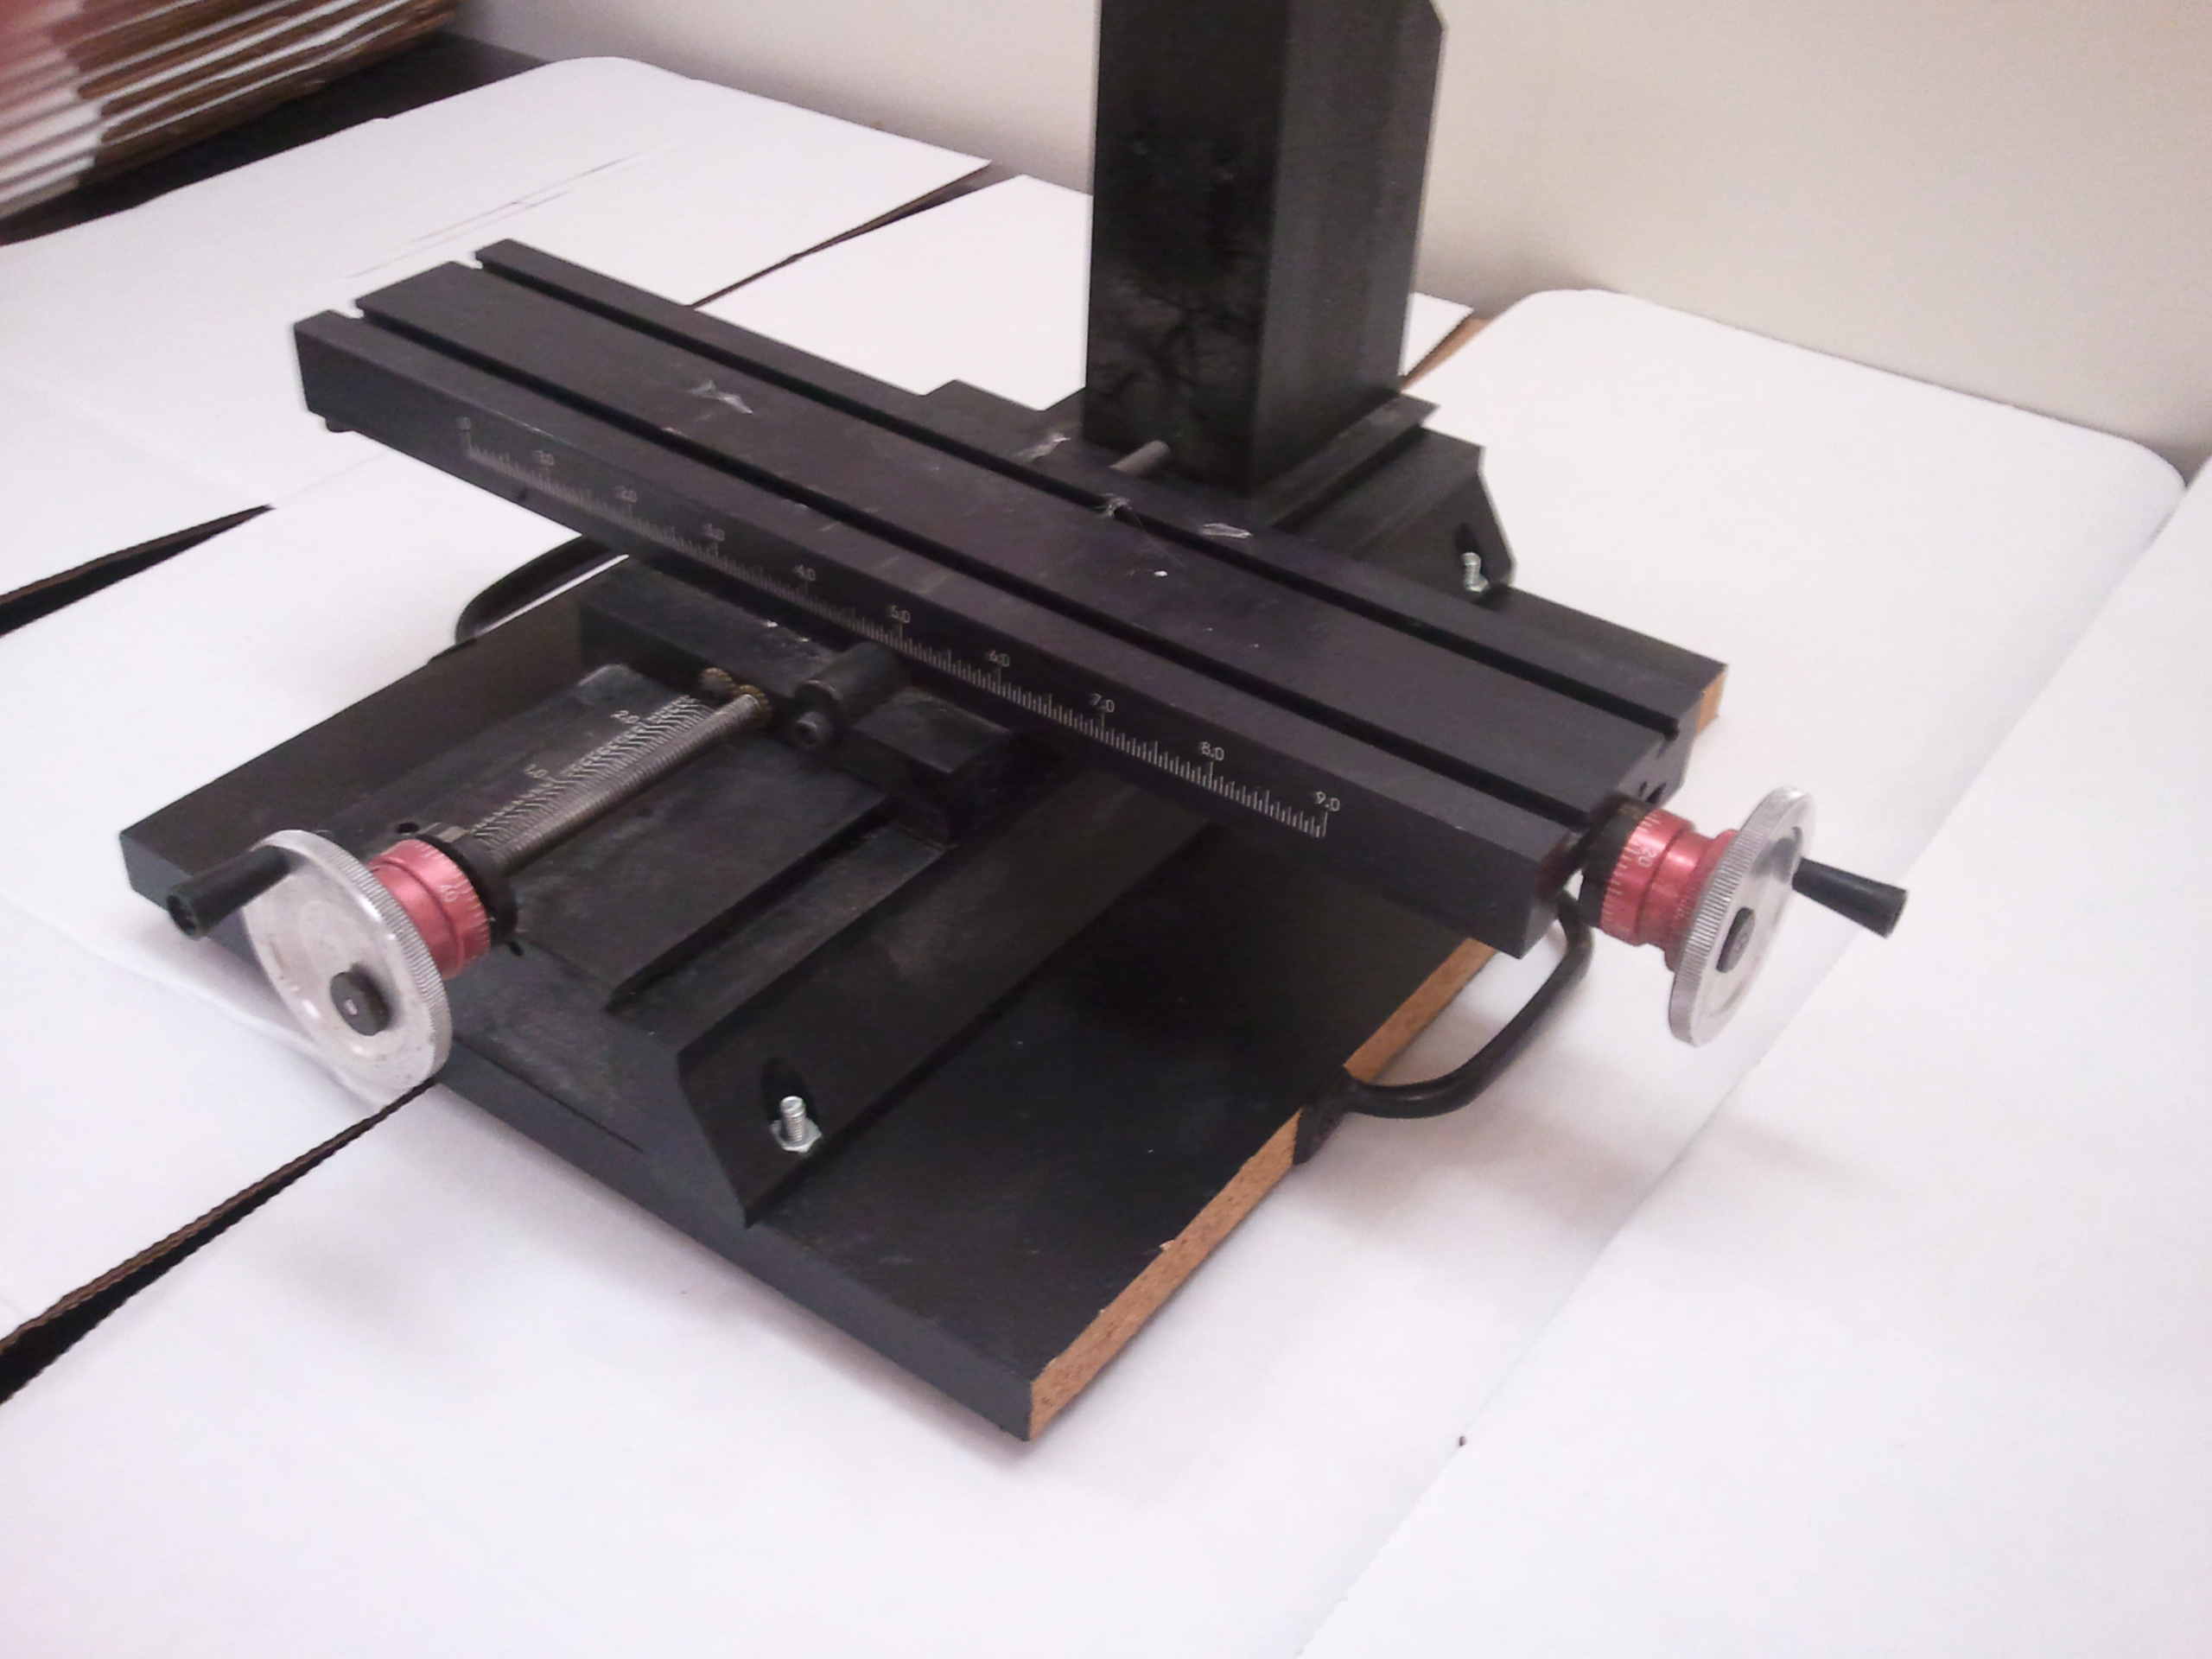
\includegraphics[width=0.5\textwidth]{img/axistable.jpg}};
    \node (knx) at (-2.7,-0.1) {};
    \node (kny) at (2,-0.5) {};
    \draw [-,dashed,ultra thick,green] (xknob.north) to[bend right] node {} (knx);
    \draw [-,dashed,ultra thick,green] (yknob.south) to[bend left] node {} (kny);

    \node (xg1) at (-1.0,-0.2) {};
    \node (xg2) at (-2.2,-1.2) {};
    \node (yg1) at (-1.7,1.5) {};
    \node (yg2) at (-3.0,2.1) {};
    \draw [<->,line width=3pt,blue] (xg1) -- node {} (xg2);
    \draw [<->,line width=3pt,blue] (yg1) -- node {} (yg2);
  \end{tikzpicture}
  \caption{Two axis table}
  \label{fig:example}
\end{figure}

\section{Model Fitting}
Input to the model comes in the form of 6D trajectories, which will be denoted by the rigid transform matrix representation, i.e. $\xse{x} = \mat{ccc|c}{&&& t_x \\ & \xmat{r} && t_y \\ &&& t_z \\\hline 0 & 0 & 0 & 1}$.\footnote{In this paper, superscripts are used for numbering object parts, feature points or graph/tree edges, while subscripts are reserved for indexing in time. Where it makes sense, operations may be considered to be implicitly vectorized (i.e. $(\xse{x}_{1..T}^a)^{-1}$ refers to $\{(\xse{x}_1^a)^{-1}, (\xse{x}_2^a)^{-1}), \dots\}$). Also, elements of $SE(3)$ will usually be shown \xsestr{} ($\xse{x}$), matrices in $\mathbb{R}^{3 \times 3}$ \xmatstr{} ($\xmat{a}$), vectors in $\mathbb{R}^2$ or $\mathbb{R}^3$ \xvecstr{} ($\xvec{v}$), and unit vectors in $\mathbb{U}^2$ or $\mathbb{U}^3$ \xuvstr{ } ($\xuv{u}$).} The full trajectory describing an object with $K$ parts over $T$ timesteps is
\begin{align}
  X = \{ \xse{x}_t^k \in SE(3) \mid k \in \{1..K\}, t \in \{1..T\} \}
\end{align}
To fit the individual joint models, the relative transformations are more useful, so for every pair of objects $a, b \in 1..K$ we will refer to the \emph{deltas}:
\begin{align}
  \xse{\Delta}_{1..T}^{a:b} &= \xse{x}_{1..T}^{b} (\xse{x}_{1..T}^{a})^{-1}
\end{align}
Using these deltas, we can treat each joint independently as if only one part is moving and the other is stationary at the origin.

\begin{figure}[ht]
  \centering
  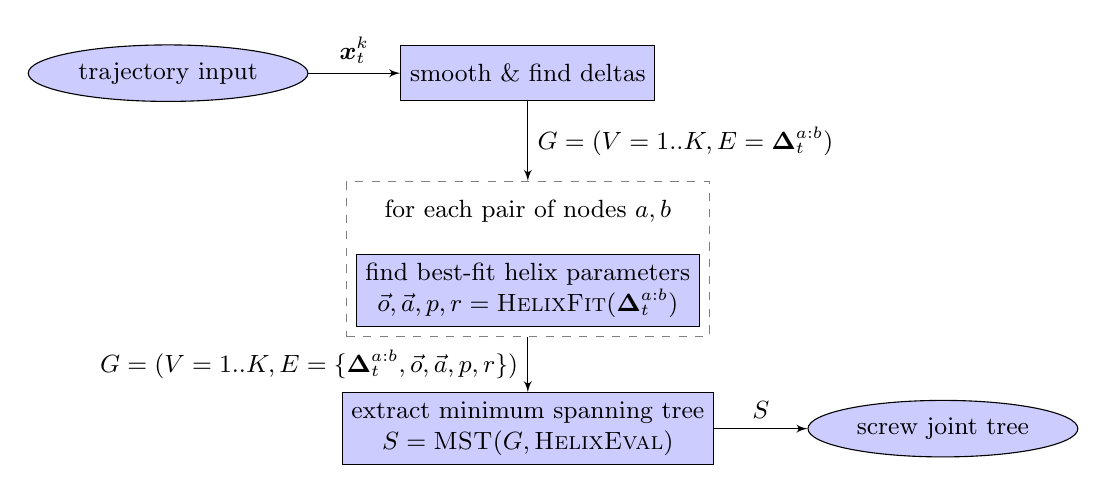
\begin{tikzpicture}[auto, >=latex']
    \tikzstyle{every node} = [font=\small]
    \tikzstyle{textbox} = [align=center, draw, fill=blue!20, minimum height=2em, minimum width=4em]
    \tikzstyle{block} = [textbox, ellipse]
    \tikzstyle{function} = [textbox, rectangle]
    \tikzstyle{pinstyle} = [pin edge={to-,thin,black}]

    \node (input) [block] {trajectory input};
    \node (preprocess) [function, right of=input, node distance=13em] {smooth \& find deltas};
    \node (loop) [below of=preprocess, node distance=5em] {for each pair of nodes $a, b$};
    \node (fit) [function, below of=loop] {find best-fit helix parameters \\ $\xvec{o}, \xvec{a}, p,r = \textsc{HelixFit}(\xse{\Delta}_t^{a:b})$};
    \node (mst) [function, below of=fit, node distance=5em] {extract minimum spanning tree \\ $S = \textsc{MST}(G, \textsc{HelixEval})$};
    \node (output) [block, right of=mst, node distance=15em] {screw joint tree};

    \node (box) [draw=black!50, dashed, fit={(loop) (fit)}] {};
    \draw [->] (input) -- node {$\xse{x}_t^k$} (preprocess);
    \draw [->] (preprocess) -- node {$G=(V=1..K, E=\xse{\Delta}_t^{a:b})$} (box);
    \draw [->] (box) -- node[left] {$G=(V=1..K, E=\{\xse{\Delta}_t^{a:b}, \xvec{o},\xvec{a},p,r\})$} (mst);
    \draw [->] (mst) -- node {$S$} (output);
  \end{tikzpicture}
  \caption{Block diagram of model fitting process}
  \label{fig:block-algo}
\end{figure}

A helix requires 8 parameters for a complete specification: the origin $\xvec{o} \in \mathbb{R}^3$, the axis $\xuv{a} \in \mathbb{U}^3$, the radius $r \in \mathbb{R}$ and pitch $p \in \mathbb{R}$. The quadratic constraint that the axis must be a unit vector means that this is a 7-dimensional configuration space. The fitting proceeds in three steps, detailed in Algorithm \ref{alg:fit}.

The first step, which is the harder and more important of the two, is to find the helix origin and axis. Our approach is to treat the trajectory as a point cloud in 3D space, and perform a principal components analysis (PCA) to find the dominant directions present in the cloud. One of the principal axes will be used as an initial estimate of the helix axis. (If the helix is long and narrow, it will be the component that describes the most variation, but we cannot assume this since the helix could be shallow, or it may not even contain a complete revolution.) We choose for the estimate the component which collapses the helix into the ``best'' circle. ``Best'' here is determined by projecting the helix down onto a plane (line \ref{alg:fit:proj}), fitting a circle (Algorithm \ref{alg:fit-findcenter}) and checking the deviation from the fitted radius (line \ref{alg:fit:ei}).

The second step, given the axis, finds the helix radius and pitch. The joint state ($\theta$) at each timestep is produced as a byproduct of this step. Our approach is to take the projected helix (produced in the first step), where it should form an arc of a circle. Then we can extract the rotation angle at each timestep (line \ref{alg:fit:atan}). This provides an estimate of the radius, and a simple linear regression (line \ref{alg:fit:linreg}) from rotation angle to height above the plane gives the pitch.

Lastly, we refine the estimates of the helix origin and axis by means of nonlinear optimization (Matlab's SQP method), contraining the axis to be a unit vector perpendicular to the origin, and using as the objective function the circularity of the helix plane projection. Then the calculations of step 2 are repeated, given the refined estimates.

\begin{algorithm}[h]
  \SetFuncSty{textsc}
  \SetProcNameSty{textsc}
  \caption{Helix Fitting Procedure}
  \label{alg:fit}
  \KwIn{$\xvec{y}_{1..T}$ relative trajectory of point $b$ (point $a$ stays at the origin)}
  \KwOut{Helix parameters $\{\xvec{o}, \xvec{a}, p, r\}$}
  \SetKwFunction{PCA}{PCA}
  \SetKwFunction{Plane}{Plane}
  \SetKwFunction{Project}{Proj}
  \SetKwFunction{LinReg}{LinReg}
  \SetKwFunction{FindCenter}{FindCenter}
  \SetKwFunction{Circularity}{Circularity}
  \SetKwFunction{Optimize}{Optimize}
  \SetKw{KwInn}{in}
  \DontPrintSemicolon
  \BlankLine

  \tcp{Step 1: find helix origin/axis}
    $\xvec{b}^{1..3}, \xvec{z}_{1..T} \leftarrow \PCA(\xvec{y}_{1..T})$ \;
    \For{$i$ \KwInn $\{1..3\}$}{
      $c \leftarrow \frac{1}{T}\sum_t \xvec{z}_t$ \;
      $c[i] \leftarrow \min_t \xvec{z}_t(i)$ \;
      $plane \leftarrow \Plane(c, b^i)$ \;
      $\xvec{u}_{1..T}^i \leftarrow \Project(plane, \xvec{y}_{1..T})$ \label{alg:fit:proj} \;
      $\xvec{o}^i, r^i \leftarrow \FindCenter(\xvec{u}_{1..T})$ \;
      $e^i \leftarrow \sum_t ( ||\xvec{u}_t - \xvec{o}^i|| )^2$ \label{alg:fit:ei} \;
    }
    $h \leftarrow \argmin_i e^i$ \;
    $\xvec{u}_{1..T}, \hat{\xvec{o}}, \hat{\xvec{a}}, \hat{r} \leftarrow \xvec{u}_{1..T}^h, \xvec{o}^h, \xvec{a}^h, r^h$ \;
  \tcp{Step 2: extrapolate angles and pitch}
    $\theta_{1..T} \leftarrow \tan^{-1}(\frac{\xvec{u}_{1..T}[2] - \hat{\xvec{o}}[2]}{\xvec{u}_{1..T}[1] - \hat{\xvec{o}}[1]})$ \label{alg:fit:atan} \;
    $\hat{p} \leftarrow \LinReg(\theta_{1..T}, \xvec{y}_{1..T} \cdot \hat{\xvec{a}})$ \label{alg:fit:linreg} \;

  \tcp{Step 3: nonlinear optimization}
    $\hat{\xvec{o}}, \hat{\xvec{a}} \leftarrow \Optimize(\Circularity(\xvec{y}_{1..T}, \xvec{o}, \xvec{a}), \xvec{o}\cdot\xvec{a}=0, ||\xvec{a}||=1, \hat{\xvec{o}}, \hat{\xvec{a}})$ \;
    $plane \leftarrow \Plane(\hat{\xvec{o}}, \hat{\xvec{a}})$ \;
    $\xvec{u}_{1..T}^i \leftarrow \Project(plane, \xvec{y}_{1..T})$ \;
    $\theta_{1..T} \leftarrow \tan^{-1}(\frac{\xvec{u}_{1..T}[2] - \hat{\xvec{o}}[2]}{\xvec{u}_{1..T}[1] - \hat{\xvec{o}}[1]})$ \;
    $\hat{p} \leftarrow \LinReg(\theta_{1..T}, \xvec{y}_{1..T} \cdot \hat{\xvec{a}})$ \;
\end{algorithm}

\begin{algorithm}[h]
  \SetFuncSty{textsc}
  \SetProcNameSty{textsc}
  \caption{\textsc{FindCenter} (subroutine for Algorithm \ref{alg:fit})}
  \label{alg:fit-findcenter}
  \KwIn{$\xvec{u}_{1..T}$ set of coplanar 2D points}
  \KwOut{$\xvec{o}$ center, $r$ radius}
  \DontPrintSemicolon
  \BlankLine

  $\xvec{a} \leftarrow \mat{cc}{\xvec{u}_{1..T} & \xvec{1}_{T \times 1}}_{T \times 3}^{-1} * \mat{c}{-||\xvec{u}_{1..T}||^2}_{T \times 1}$ \;
  $\xvec{o} \leftarrow \mat{cc}{\xvec{a}[1] & \xvec{a}[2]}$ \;
  $r \leftarrow \xvec{a}[3]$ \;

\end{algorithm}

\begin{algorithm}[h]
  \SetFuncSty{textsc}
  \SetProcNameSty{textsc}
  \caption{\textsc{Circularity} (subroutine for Algorithm \ref{alg:fit})}
  \label{alg:fit-circularity}
  \KwIn{$\xvec{y}_{1..T}$ set of 3D points, $\xvec{o}$ plane origin, $\xvec{a}$ plane normal}
  \KwOut{$e$ circularity score}
  \SetKwFunction{Plane}{Plane}
  \SetKwFunction{Project}{Proj}
  \SetKwFunction{FindCenter}{FindCenter}
  \SetKwFunction{Std}{Std}
  \DontPrintSemicolon
  \BlankLine

  $plane \leftarrow \Plane(\xvec{o}, \xvec{a})$ \;
  $\xvec{u}_{1..T} \leftarrow \Project(plane, \xvec{y}_{1..T})$ \;
  $\xvec{o} \leftarrow \FindCenter(\xvec{u}_{1..T})$ \;
  $e \leftarrow \Std( \sum_t || \xvec{u}_t - \xvec{o} || )$ \;

\end{algorithm}

\section{Evaluation}
The helix fitting system has been evaluted both in simulation and using real-world data captured from the swivel chair pictured in Figure \ref{fig:chair} (which is, despite its mundane nature, a quite kinematically versatile object).

\subsection{Simulation}

The goal of the simulation experiment is to define a screw joint by its parameters, and generate a trajectory by executing a random walk in state space. At this point noise is added, and we hope to recover the original helix parameters from the noisy trajectory by Algorithm \ref{alg:fit}.

The forward kinematics of a screw joint, as applied to a vector $\xvec{v}$, are given by the following chain of rigid transformations, read from right to left. First, $\xse{c}$ moves the origin to the helix origin and aligns the $z$-axis with the helix axis. \textsc{T} and \textsc{R} generate pure translation and rotation about the $z$-axis. Then $\xse{r}$ incorporates the helix radius.
\begin{align}
  \xse{s}*\xvec{v} &= \xse{r} * \textsc{R}(\mat{ccc}{0 & 0 & \theta}) * \textsc{T}(\mat{ccc}{0 & 0 & \theta p}) * \xse{c} * \xvec{v}
\end{align}
With two rigid transformations, plus the pitch, totaling 13 parameters, this representation is richer than the 7-dimensional description of a helix given earlier. This is due to the fact that $\xse{r}$ can incorporate an arbitrary post-transformation as long as it maintains a constant helix radius, and $\xse{c}$ must align the $z$-axis but may rotate the $xy$-plane. This accounts for the extra 6 parameters. Though the full parametrization follows the pattern of \cite{Burka2013} and is necessary for modeling general kinematic chains without resorting to intermediate rigid joints, here for the purposes of simulation we will restrict $\xse{c}$ to a simple translation and rotation, and $\xse{r}$ to a one-dimensional translation.

The simulator is controlled by a graphical interface which also grew out of the system presented in \cite{Burka2013}, shown in Figure \ref{fig:gui}. It contains a tree editor and can simulate arbitrary kinematic chains of rigid, prismatic, revolute and screw joints (the last was added for this work). The source code and data files used to generate the simulated trajectories used here can be found in Appendix \ref{sec:code}.

\begin{figure}[ht]
  \centering
  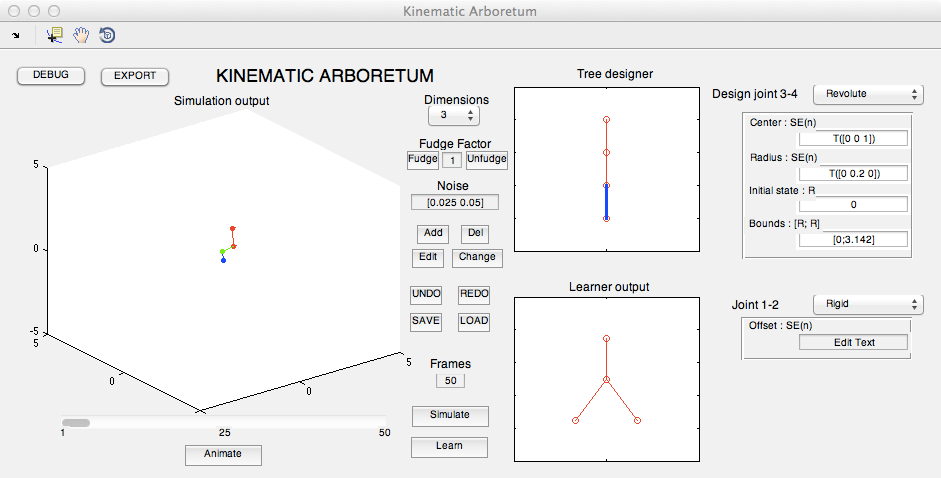
\includegraphics[width=.9\textwidth]{img/screenshot.png}
  \caption{Custom GUI for designing and simulating articulated objects}
  \label{fig:gui}
\end{figure}

For this experiment, two screw joints were simulated. Both have an origin at $(0, 0, 0)$, a helix axis of $(0, 0, 1)$ and a radius of 1. One joint has a pitch of 0 (making it a revolute joint) and the other has a pitch of 5. Table \ref{tbl:simulation} shows the learned parameters and Figure \ref{fig:simulation} shows a representation of the results.

\begin{table}[ht]
  \begin{tabular}{c|c|c|c|c}
           & \multicolumn{2}{c}{Revolute} & \multicolumn{2}{|c}{Screw} \\
           & Simulated   & Detected    & Simulated   & Detected    \\ \hline
    Origin & $(0, 0, 0)$ & $(0.0005, -0.0065, 0.0008)$ & $(0, 0, 0)$ & $(0.2682, 0.2546, -0.0011)$ \\
    Axis   & $(0, 0, 1)$ & $(-0.0654, 0.1154, 0.9912)$ & $(0, 0, 1)$ & $(0.0035, 0.0006, 1.000)$ \\
    Radius & 1           & 1.5583      & 1           & 1.0980      \\
    Pitch  & 0           & 0.0175      & 5           & 4.9240      \\
  \end{tabular}
  \caption{Parameters through the simulation}
  \label{tbl:simulation}
\end{table}

\subsection{Swivel Chair}
The first experiment focused on a common swivel chair (pictured at left in Figure \ref{fig:chair}) as the articulated object of interest. In particular, between the base and the seat there is a prismatic/revolute joint with two degrees of freedom. This makes the chair a versatile object in the context of our system which models 1-DOF joints. Depending on the type of motion performed during the recording (videos available; see Section \ref{sec:code}), the chair can appear as a pure prismatic joint, a pure revolute joint, or a screw joint.\footnote{Since the joint actually has two degrees of freedom, it has no fixed pitch. Therefore, making a screw joint for recording purposes requires a steady hand. See the video for details.}

\begin{figure}[ht]
  \centering
  \begin{tikzpicture}
    \node (image) {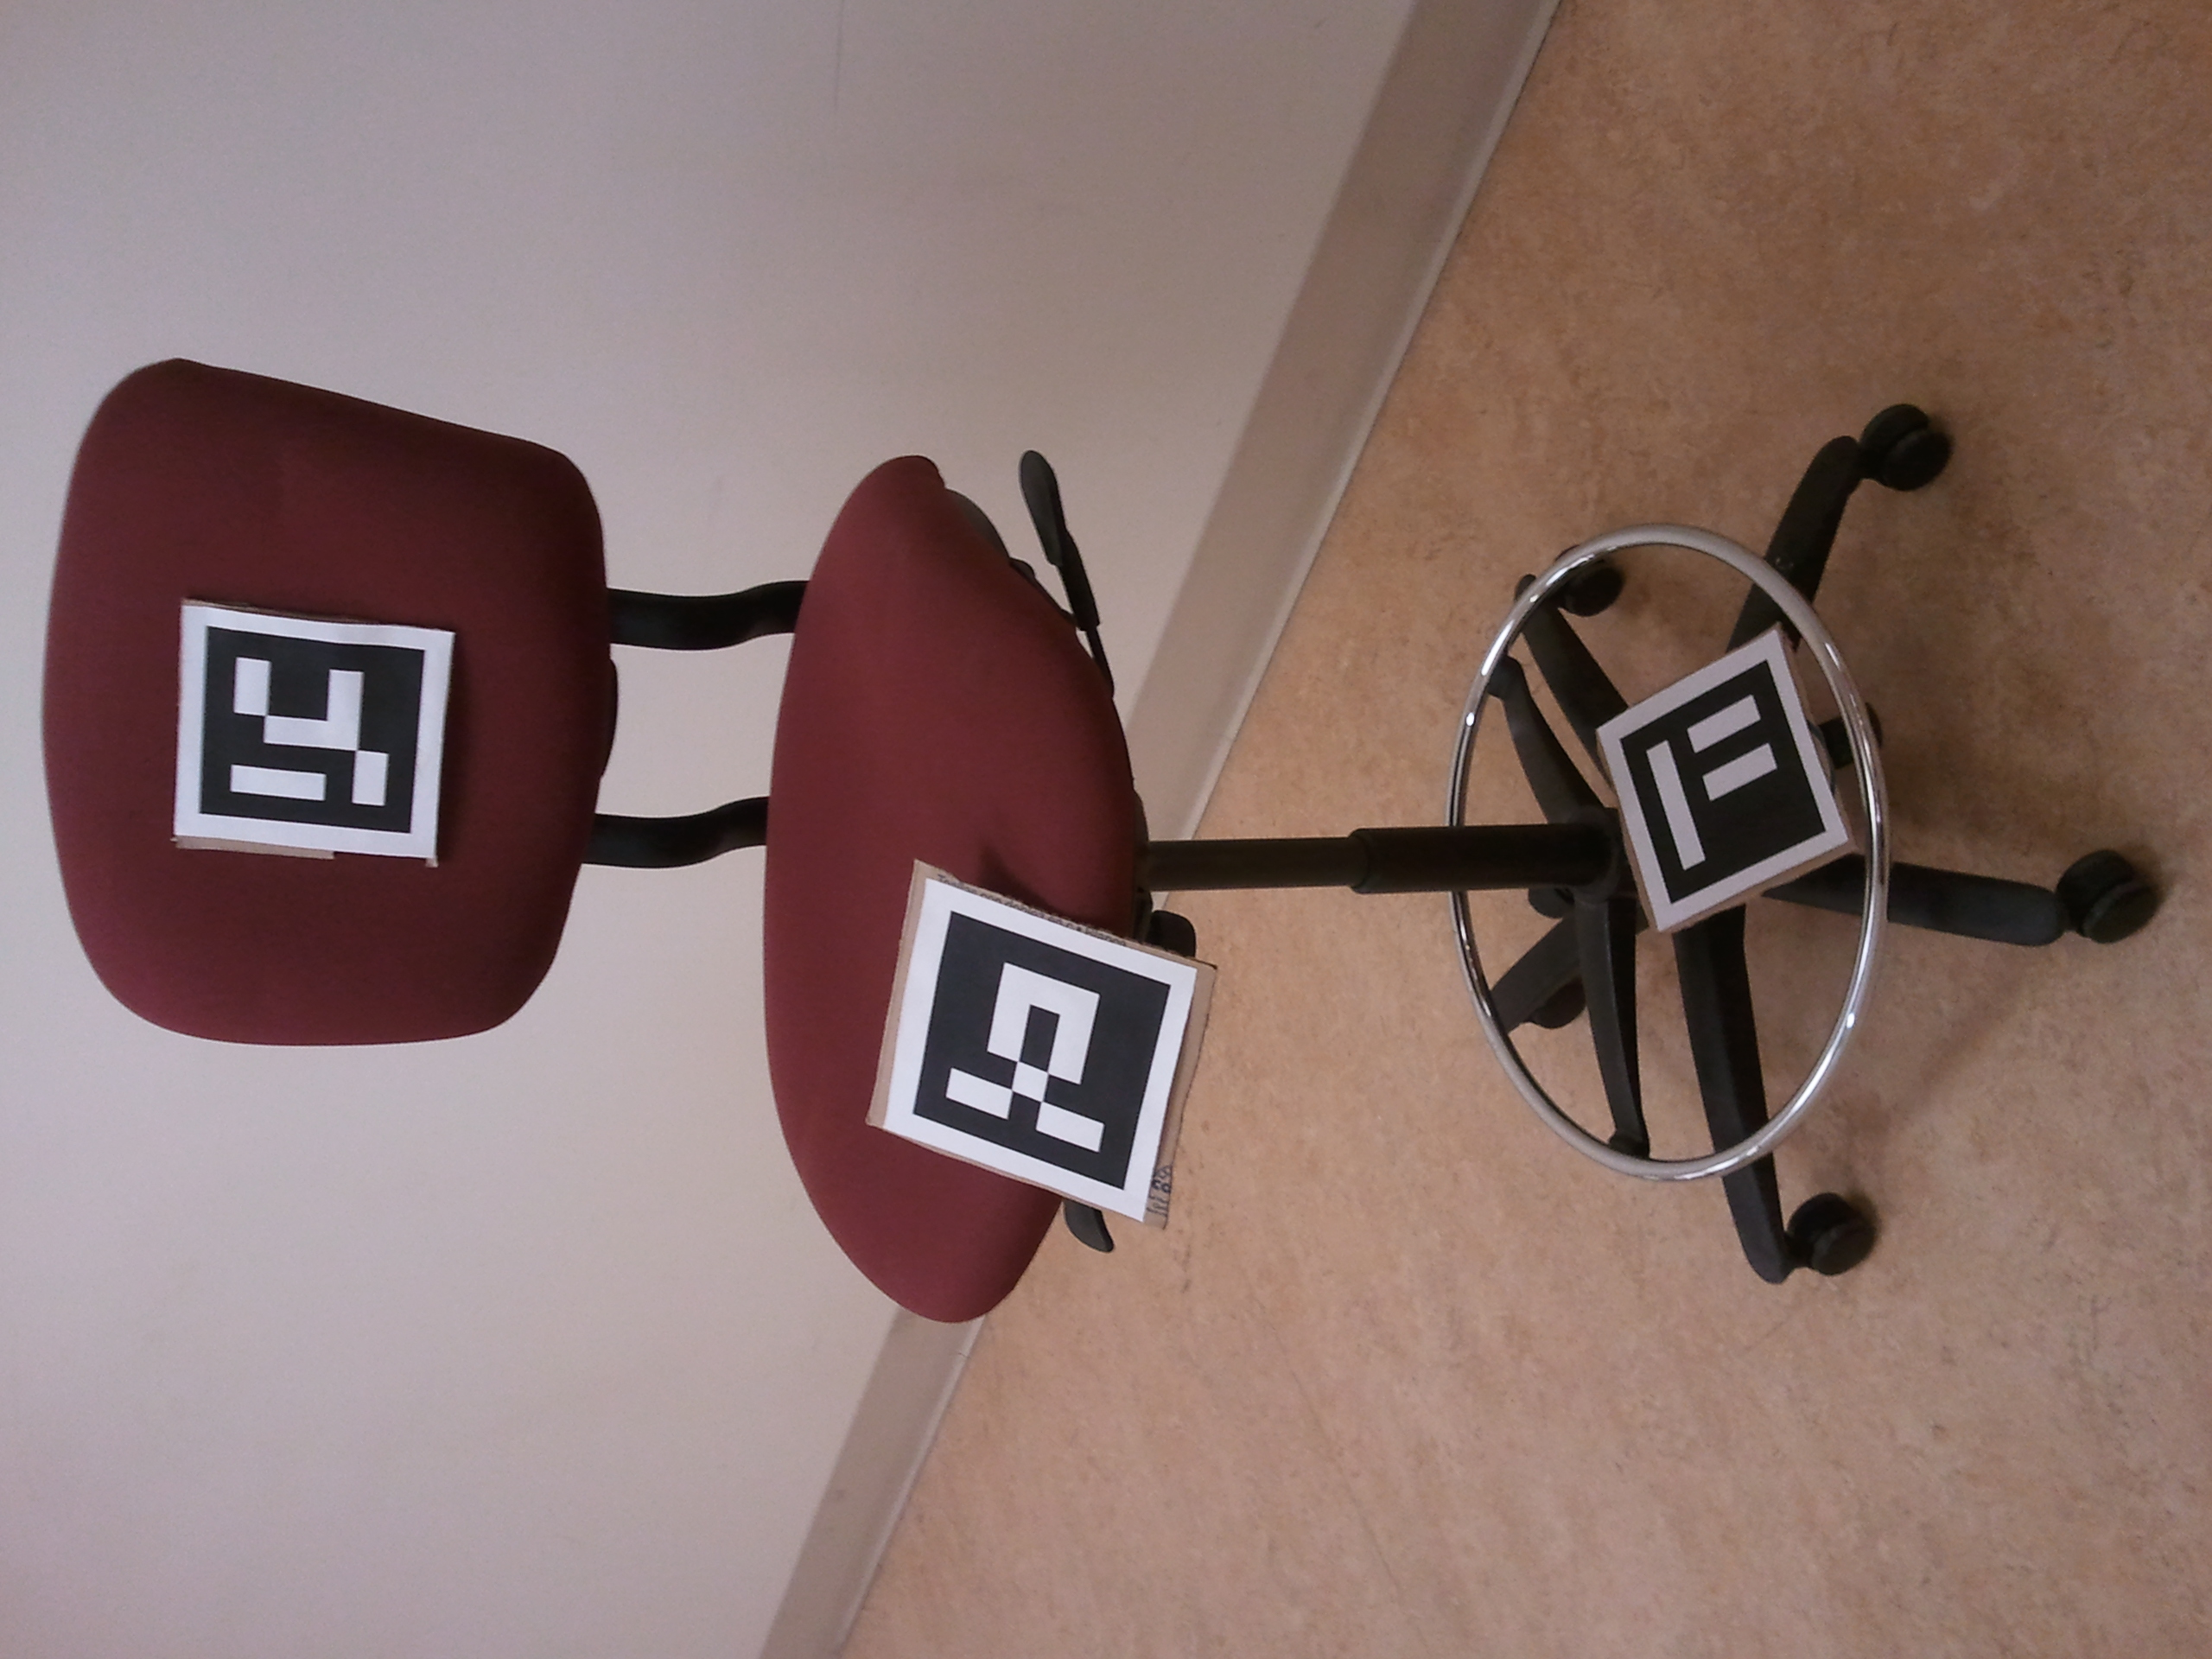
\includegraphics[width=0.5\textwidth,angle=-90]{img/chair.jpg}};
    \node (chair2) at (6,1.75) {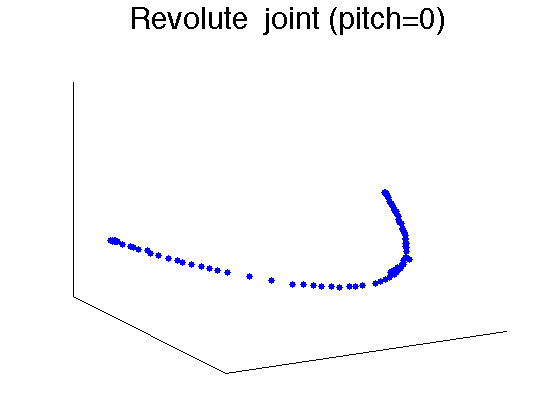
\includegraphics[width=0.3\textwidth]{img/chair2.png}};
    \node (chair2) at (6,-1.75) {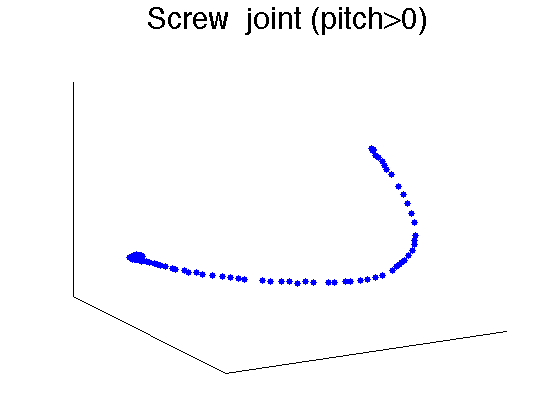
\includegraphics[width=0.3\textwidth]{img/chair3.png}};
  \end{tikzpicture}
  \caption{Swivel chair instrumented with Aruco tags}
  \label{fig:chair}
\end{figure}

\section{Conclusions and Future Work}

\appendix

\section{Source Code}

\section{Submission of papers to NIPS 2013}

NIPS requires electronic submissions.  The electronic submission site is  
\begin{center}
   \url{http://papers.nips.cc}
\end{center}

Please read carefully the
instructions below, and follow them faithfully.
\subsection{Style}

Papers to be submitted to NIPS 2013 must be prepared according to the
instructions presented here. Papers may be only up to eight pages long,
including figures. Since 2009 an additional ninth page \textit{containing only
cited references} is allowed. Papers that exceed nine pages will not be
reviewed, or in any other way considered for presentation at the conference.
%This is a strict upper bound. 

Please note that this year we have introduced automatic line number generation
into the style file (for \LaTeXe and Word versions). This is to help reviewers
refer to specific lines of the paper when they make their comments. Please do
NOT refer to these line numbers in your paper as they will be removed from the
style file for the final version of accepted papers.

The margins in 2013 are the same as since 2007, which allow for $\approx 15\%$
more words in the paper compared to earlier years. We are also again using 
double-blind reviewing. Both of these require the use of new style files.

Authors are required to use the NIPS \LaTeX{} style files obtainable at the
NIPS website as indicated below. Please make sure you use the current files and
not previous versions. Tweaking the style files may be grounds for rejection.

%% \subsection{Double-blind reviewing}

%% This year we are doing double-blind reviewing: the reviewers will not know 
%% who the authors of the paper are. For submission, the NIPS style file will 
%% automatically anonymize the author list at the beginning of the paper.

%% Please write your paper in such a way to preserve anonymity. Refer to
%% previous work by the author(s) in the third person, rather than first
%% person. Do not provide Web links to supporting material at an identifiable
%% web site.

%%\subsection{Electronic submission}
%%
%% \textbf{THE SUBMISSION DEADLINE IS MAY 31st, 2013. SUBMISSIONS MUST BE LOGGED BY
%% 23:00, MAY 31st, 2013, UNIVERSAL TIME}

%% You must enter your submission in the electronic submission form available at
%% the NIPS website listed above. You will be asked to enter paper title, name of
%% all authors, keyword(s), and data about the contact
%% author (name, full address, telephone, fax, and email). You will need to
%% upload an electronic (postscript or pdf) version of your paper.

%% You can upload more than one version of your paper, until the
%% submission deadline. We strongly recommended uploading your paper in
%% advance of the deadline, so you can avoid last-minute server congestion.
%%
%% Note that your submission is only valid if you get an e-mail
%% confirmation from the server. If you do not get such an e-mail, please
%% try uploading again. 


\subsection{Retrieval of style files}

The style files for NIPS and other conference information are available on the World Wide Web at
\begin{center}
   \url{http://www.nips.cc/}
\end{center}
The file \verb+nips2013.pdf+ contains these 
instructions and illustrates the
various formatting requirements your NIPS paper must satisfy. \LaTeX{}
users can choose between two style files:
\verb+nips11submit_09.sty+ (to be used with \LaTeX{} version 2.09) and
\verb+nips11submit_e.sty+ (to be used with \LaTeX{}2e). The file
\verb+nips2013.tex+ may be used as a ``shell'' for writing your paper. All you
have to do is replace the author, title, abstract, and text of the paper with
your own. The file
\verb+nips2013.rtf+ is provided as a shell for MS Word users.

The formatting instructions contained in these style files are summarized in
sections \ref{gen_inst}, \ref{headings}, and \ref{others} below.

%% \subsection{Keywords for paper submission}
%% Your NIPS paper can be submitted with any of the following keywords (more than one keyword is possible for each paper):

%% \begin{verbatim}
%% Bioinformatics
%% Biological Vision
%% Brain Imaging and Brain Computer Interfacing
%% Clustering
%% Cognitive Science
%% Control and Reinforcement Learning
%% Dimensionality Reduction and Manifolds
%% Feature Selection
%% Gaussian Processes
%% Graphical Models
%% Hardware Technologies
%% Kernels
%% Learning Theory
%% Machine Vision
%% Margins and Boosting
%% Neural Networks
%% Neuroscience
%% Other Algorithms and Architectures
%% Other Applications
%% Semi-supervised Learning
%% Speech and Signal Processing
%% Text and Language Applications

%% \end{verbatim}

\section{General formatting instructions}
\label{gen_inst}

The text must be confined within a rectangle 5.5~inches (33~picas) wide and
9~inches (54~picas) long. The left margin is 1.5~inch (9~picas).
Use 10~point type with a vertical spacing of 11~points. Times New Roman is the
preferred typeface throughout. Paragraphs are separated by 1/2~line space,
with no indentation.

Paper title is 17~point, initial caps/lower case, bold, centered between
2~horizontal rules. Top rule is 4~points thick and bottom rule is 1~point
thick. Allow 1/4~inch space above and below title to rules. All pages should
start at 1~inch (6~picas) from the top of the page.

%The version of the paper submitted for review should have ``Anonymous Author(s)'' as the author of the paper.

For the final version, authors' names are
set in boldface, and each name is centered above the corresponding
address. The lead author's name is to be listed first (left-most), and
the co-authors' names (if different address) are set to follow. If
there is only one co-author, list both author and co-author side by side.

Please pay special attention to the instructions in section \ref{others}
regarding figures, tables, acknowledgments, and references.

\section{Headings: first level}
\label{headings}

First level headings are lower case (except for first word and proper nouns),
flush left, bold and in point size 12. One line space before the first level
heading and 1/2~line space after the first level heading.

\subsection{Headings: second level}

Second level headings are lower case (except for first word and proper nouns),
flush left, bold and in point size 10. One line space before the second level
heading and 1/2~line space after the second level heading.

\subsubsection{Headings: third level}

Third level headings are lower case (except for first word and proper nouns),
flush left, bold and in point size 10. One line space before the third level
heading and 1/2~line space after the third level heading.

\section{Citations, figures, tables, references}
\label{others}

These instructions apply to everyone, regardless of the formatter being used.

\subsection{Citations within the text}

Citations within the text should be numbered consecutively. The corresponding
number is to appear enclosed in square brackets, such as [1] or [2]-[5]. The
corresponding references are to be listed in the same order at the end of the
paper, in the \textbf{References} section. (Note: the standard
\textsc{Bib\TeX} style \texttt{unsrt} produces this.) As to the format of the
references themselves, any style is acceptable as long as it is used
consistently.

As submission is double blind, refer to your own published work in the 
third person. That is, use ``In the previous work of Jones et al.\ [4]'',
not ``In our previous work [4]''. If you cite your other papers that
are not widely available (e.g.\ a journal paper under review), use
anonymous author names in the citation, e.g.\ an author of the
form ``A.\ Anonymous''. 


\subsection{Footnotes}

Indicate footnotes with a number\footnote{Sample of the first footnote} in the
text. Place the footnotes at the bottom of the page on which they appear.
Precede the footnote with a horizontal rule of 2~inches
(12~picas).\footnote{Sample of the second footnote}

\subsection{Figures}

All artwork must be neat, clean, and legible. Lines should be dark
enough for purposes of reproduction; art work should not be
hand-drawn. The figure number and caption always appear after the
figure. Place one line space before the figure caption, and one line
space after the figure. The figure caption is lower case (except for
first word and proper nouns); figures are numbered consecutively.

Make sure the figure caption does not get separated from the figure.
Leave sufficient space to avoid splitting the figure and figure caption.

You may use color figures. 
However, it is best for the
figure captions and the paper body to make sense if the paper is printed
either in black/white or in color.
\begin{figure}[h]
\begin{center}
%\framebox[4.0in]{$\;$}
\fbox{\rule[-.5cm]{0cm}{4cm} \rule[-.5cm]{4cm}{0cm}}
\end{center}
\caption{Sample figure caption.}
\end{figure}

\subsection{Tables}

All tables must be centered, neat, clean and legible. Do not use hand-drawn
tables. The table number and title always appear before the table. See
Table~\ref{sample-table}.

Place one line space before the table title, one line space after the table
title, and one line space after the table. The table title must be lower case
(except for first word and proper nouns); tables are numbered consecutively.

\begin{table}[t]
\caption{Sample table title}
\label{sample-table}
\begin{center}
\begin{tabular}{ll}
\multicolumn{1}{c}{\bf PART}  &\multicolumn{1}{c}{\bf DESCRIPTION}
\\ \hline \\
Dendrite         &Input terminal \\
Axon             &Output terminal \\
Soma             &Cell body (contains cell nucleus) \\
\end{tabular}
\end{center}
\end{table}

\section{Final instructions}
Do not change any aspects of the formatting parameters in the style files.
In particular, do not modify the width or length of the rectangle the text
should fit into, and do not change font sizes (except perhaps in the
\textbf{References} section; see below). Please note that pages should be
numbered.

\section{Preparing PostScript or PDF files}

Please prepare PostScript or PDF files with paper size ``US Letter'', and
not, for example, ``A4''. The -t
letter option on dvips will produce US Letter files.

Fonts were the main cause of problems in the past years. Your PDF file must
only contain Type 1 or Embedded TrueType fonts. Here are a few instructions
to achieve this.

\begin{itemize}

\item You can check which fonts a PDF files uses.  In Acrobat Reader,
select the menu Files$>$Document Properties$>$Fonts and select Show All Fonts. You can
also use the program \verb+pdffonts+ which comes with \verb+xpdf+ and is
available out-of-the-box on most Linux machines.

\item The IEEE has recommendations for generating PDF files whose fonts
are also acceptable for NIPS. Please see
\url{http://www.emfield.org/icuwb2010/downloads/IEEE-PDF-SpecV32.pdf}

\item LaTeX users:

\begin{itemize}

\item Consider directly generating PDF files using \verb+pdflatex+
(especially if you are a MiKTeX user). 
PDF figures must be substituted for EPS figures, however.

\item Otherwise, please generate your PostScript and PDF files with the following commands:
\begin{verbatim} 
dvips mypaper.dvi -t letter -Ppdf -G0 -o mypaper.ps
ps2pdf mypaper.ps mypaper.pdf
\end{verbatim}

Check that the PDF files only contains Type 1 fonts. 
%For the final version, please send us both the Postscript file and
%the PDF file. 

\item xfig "patterned" shapes are implemented with 
bitmap fonts.  Use "solid" shapes instead. 
\item The \verb+\bbold+ package almost always uses bitmap
fonts.  You can try the equivalent AMS Fonts with command
\begin{verbatim}
\usepackage[psamsfonts]{amssymb}
\end{verbatim}
 or use the following workaround for reals, natural and complex: 
\begin{verbatim}
\newcommand{\RR}{I\!\!R} %real numbers
\newcommand{\Nat}{I\!\!N} %natural numbers 
\newcommand{\CC}{I\!\!\!\!C} %complex numbers
\end{verbatim}

\item Sometimes the problematic fonts are used in figures
included in LaTeX files. The ghostscript program \verb+eps2eps+ is the simplest
way to clean such figures. For black and white figures, slightly better
results can be achieved with program \verb+potrace+.
\end{itemize}
\item MSWord and Windows users (via PDF file):
\begin{itemize}
\item Install the Microsoft Save as PDF Office 2007 Add-in from
\url{http://www.microsoft.com/downloads/details.aspx?displaylang=en\&familyid=4d951911-3e7e-4ae6-b059-a2e79ed87041}
\item Select ``Save or Publish to PDF'' from the Office or File menu
\end{itemize}
\item MSWord and Mac OS X users (via PDF file):
\begin{itemize}
\item From the print menu, click the PDF drop-down box, and select ``Save
as PDF...''
\end{itemize}
\item MSWord and Windows users (via PS file):
\begin{itemize}
\item To create a new printer
on your computer, install the AdobePS printer driver and the Adobe Distiller PPD file from
\url{http://www.adobe.com/support/downloads/detail.jsp?ftpID=204} {\it Note:} You must reboot your PC after installing the
AdobePS driver for it to take effect.
\item To produce the ps file, select ``Print'' from the MS app, choose
the installed AdobePS printer, click on ``Properties'', click on ``Advanced.''
\item Set ``TrueType Font'' to be ``Download as Softfont''
\item Open the ``PostScript Options'' folder
\item Select ``PostScript Output Option'' to be ``Optimize for Portability''
\item Select ``TrueType Font Download Option'' to be ``Outline''
\item Select ``Send PostScript Error Handler'' to be ``No''
\item Click ``OK'' three times, print your file.
\item Now, use Adobe Acrobat Distiller or ps2pdf to create a PDF file from
the PS file. In Acrobat, check the option ``Embed all fonts'' if
applicable.
\end{itemize}

\end{itemize}
If your file contains Type 3 fonts or non embedded TrueType fonts, we will
ask you to fix it. 

\subsection{Margins in LaTeX}
 
Most of the margin problems come from figures positioned by hand using
\verb+\special+ or other commands. We suggest using the command
\verb+\includegraphics+
from the graphicx package. Always specify the figure width as a multiple of
the line width as in the example below using .eps graphics
\begin{verbatim}
   \usepackage[dvips]{graphicx} ... 
   \includegraphics[width=0.8\linewidth]{myfile.eps} 
\end{verbatim}
or % Apr 2009 addition
\begin{verbatim}
   \usepackage[pdftex]{graphicx} ... 
   \includegraphics[width=0.8\linewidth]{myfile.pdf} 
\end{verbatim}
for .pdf graphics. 
See section 4.4 in the graphics bundle documentation (\url{http://www.ctan.org/tex-archive/macros/latex/required/graphics/grfguide.ps}) 
 
A number of width problems arise when LaTeX cannot properly hyphenate a
line. Please give LaTeX hyphenation hints using the \verb+\-+ command.


\subsubsection*{Acknowledgments}

Use unnumbered third level headings for the acknowledgments. All
acknowledgments go at the end of the paper. Do not include 
acknowledgments in the anonymized submission, only in the 
final paper. 


\bibliographystyle{plain}
\renewcommand{\refname}{\vspace{-2.5em}\subsubsection*{References}}
{\small
\bibliography{research}
}

\end{document}
